\subsection{Noether 环上的 m-进拓扑}

命题 4。设 A 为交换 Noether 环，m 为 A 的理想，E 为有限生成的 A-模。E 上所有 m-好滤过定义同一个拓扑（即 m-进拓扑）。

设 \((\mathbf{E}_{n})\) 是 E 上的 m-好滤过。由于此滤过是穷竭的，E 的每个元素都属于某个 \(E_{n}\)；又因 E 有限生成且各 \(E_{n}\) 都是 A-模，存在整数 \(n_{1}\)，使得 \(E_{n_{1}} = E\)。另一方面，取 \(n_{0}\) 使得 \(mE_{n} = E_{n+1}\) 对 \(n \geqslant n_{0}\) 成立；于是当 \(n > n_{0} - n_{1}\) 时，\(m^{n}E \subset E_{n+n_{1}} = m^{n+n_{1}-n_{0}}E_{n_{0}} \subset m^{n+n_{1}-n_{0}}E\)，这就证明了命题。

定理 2（Krull）。设 A 为交换 Noether 环，m 为 A 的理想，E 为有限生成的 A-模，F 为 E 的子模。则 F 上的 m-进拓扑由 E 上的 m-进拓扑诱导。

由第 1 号命题 1，E 上的 m-进滤过在 F 上诱导的滤过是 m-好的，结论于是由命题 4 得出。

推论。设 A 为交换 Noether 环，m 为 A 的理想，E 为 A-模，F 为有限生成的 A-模。对于 m-进拓扑，任意 A-线性映射 u: E → F 都是严格态射（一般拓扑学，第三章，第 2 节，第 8 号）。

由于 \(u(\mathfrak{m}^{n}\mathbf{E}) = \mathfrak{m}^{n}u(\mathbf{E})\)，对于这两个模上的 m-进拓扑，u 是从 E 到 \(u(\mathbf{E})\) 的严格态射；又根据定理 2，\(u(\mathbf{E})\) 上的 m-进拓扑由 F 上的 m-进拓扑诱导。

命题 5。设 A 为交换 Noether 环，m 为 A 的理想，E 为有限生成的 A-模。关于 m-进拓扑，E 中由 \(\bigcap_{n=1}^{\infty} \mathfrak{m}^{n}\mathrm{E}\) 给出的 \(\{0\}\) 的闭包是所有满足如下条件的 \(x \in \mathrm{E}\) 的集合：存在 \(m \in \mathfrak{m}\)，使得 \((1 - m)x = 0\)。若 \(x = mx\)，其中 \(m \in \mathfrak{m}\)，则 \(x = m^{n}x \in \mathfrak{m}^{n}\mathrm{E}\) 对每个整数 \(n \geqslant 0\) 都成立，因而 \(x \in \mathrm{F} = \bigcap_{n=0}^{\infty} \mathfrak{m}^{n}\mathrm{E}\)。反之，若 \(x \in \mathrm{F}\)，则 Ax 包含于 E 中 0 的邻域的交；于是由定理 2，Ax 上由 E 上的拓扑诱导的 m-进拓扑是最粗拓扑；按定义 mx 是此拓扑下 0 的一个邻域，所以 mx = Ax，从而存在 \(m \in \mathfrak{m}\)，使得 \(x = mx\)。

由于

\[
\mathrm{F} = \bigcap_ {n = 1} ^ {\infty} m ^ {n + 1} \mathrm{E} \subset m. \bigcap_ {n = 1} ^ {\infty} m ^ {n} \mathrm{E} = m \mathrm{F};
\]

由于 A 是 Noether 环，F 是有限生成的 A-模；于是只需将第二章第 2 节第 2 号命题 4 的推论 3 应用于此处。

推论（Krull）。设 A 为交换 Noether 环，m 为 A 的理想。理想 \(\bigcap_{n=1}^{\infty}m^{n}\) 是所有满足如下条件的元素 \(x\in A\) 的集合：存在 \(m\in m\)，使得 \((1-m)x=0\)。特别地，当 \(\bigcap_{n=1}^{\infty}m^{n}=\{0\}\) 时，其充要条件是 \(1+m\) 中没有元素是 A 的零因子。

只需将命题 5 应用于 \(\mathbf{E} = \mathbf{A}_s\)。

\pandocbounded{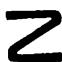
\includegraphics[keepaspectratio]{images/part002_69a966b6.jpg}}

注。A 为 Noether 环这一假设对于本推论是必要的。例如，设 A 是从 R 到自身的无穷可微映射组成的环，m 是 A 的由满足 \(f(0) = 0\) 的函数 f 组成的（极大）理想。立即可见，\(\bigcap_{n=0}^{\infty} m^{n}\) 是满足下述条件的函数 f 的集合：

\(f^{(n)}(0) = 0\) 对所有 \(n \geqslant 0\) 都成立；并且存在满足此条件而对所有 \(f(x) \neq 0\) 的 \(x \neq 0\) 都成立的函数，例如函数 \(f\)，它由 \(f(x) = e^{-1 / x^2}\)（\(x \neq 0\)）定义，且 \(f(0) = 0\)。

定义 1。设 A 为拓扑环。若 A 的一个双边理想 m 使得 A 上给定的拓扑是 m-进拓扑，则称 m 为 A 上该拓扑的定义理想。

设 A 为交换 Noether 环，m 为 A 的理想，t 为其根（第二章，第 2 节，第 6 号）。若 \(m'\) 是 m-进拓扑的定义理想，则存在整数 n \textgreater{} 0，使得 \(m'^{n} \subset m\)（第 2 节，第 5 号），因而 \(m' \subset t\)；反之，由于 A 是 Noether 环，存在整数 k \textgreater{} 0，使得 \(t^{k} \subset m\)（第二章，第 2 节，第 6 号，命题 15），因而 t 是 m-进拓扑的最大定义理想。

